\documentclass[a4paper,11pt]{article}

\usepackage{graphicx,epsfig,subfig}
\usepackage{fancyhdr,fancybox}
\usepackage{indentfirst}
\usepackage{titlesec}
\usepackage{verbatim}
\usepackage[titletoc,title]{appendix}
\usepackage[sort&compress, numbers]{natbib}
\usepackage{array,dcolumn,tabularx}
\usepackage{setspace}
\usepackage{geometry}
\usepackage{extarrows,chemarrow,xypic}
\usepackage{lineno}
\usepackage{microtype}
\usepackage{xcolor}

\usepackage{latexsym}
\usepackage{amsmath}
\usepackage{amssymb}
\usepackage{amsbsy}
\usepackage{amsthm}
\usepackage{amsfonts}
\usepackage{mathrsfs}
\usepackage{bm}
\usepackage{arydshln}
\usepackage{relsize}
\usepackage{hyperref}

%\renewcommand{\rmdefault}{ptm}
\newcommand{\paperfont}{\fontsize{11pt}{1.2\baselineskip}\selectfont}
\geometry{top=1in,bottom=1in,left=1in,right=1in}
\parindent 4ex


\begin{document}

\theoremstyle{definition}
\makeatletter
\thm@headfont{\bf}
\makeatother
\newtheorem{definition}{Definition}
\newtheorem{example}{Example}
\newtheorem{theorem}{Theorem}
\newtheorem{lemma}{Lemma}
\newtheorem{corollary}{Corollary}
\newtheorem{remark}{Remark}
\newtheorem{proposition}{Proposition}

\lhead{}
\rhead{}
\lfoot{}
\rfoot{}

\renewcommand{\refname}{References}
\renewcommand{\figurename}{Fig.}
\renewcommand{\tablename}{Table}
\renewcommand{\proofname}{Proof}

\newcommand{\diag}{\mathrm{diag}}
\newcommand{\tr}{\mathrm{tr}}
\newcommand{\dnum}{\mathrm{d}}
\newcommand{\Enum}{\mathbb{E}}
\newcommand{\Pnum}{\mathbb{P}}
\newcommand{\Rnum}{\mathbb{R}}
\newcommand{\Cnum}{\mathbb{C}}
\newcommand{\Znum}{\mathbb{Z}}
\newcommand{\Nnum}{\mathbb{N}}
\newcommand{\abs}[1]{\left\vert#1\right\vert}
\newcommand{\set}[1]{\left\{#1\right\}}
\newcommand{\norm}[1]{\left\Vert#1\right\Vert}
\newcommand{\Q}{\boldsymbol{Q}}
\newcommand{\W}{\boldsymbol{W}}
\newcommand{\I}{\boldsymbol{I}}
\newcommand{\M}{\boldsymbol{M}}
\newcommand{\p}{\boldsymbol{p}}
\newcommand{\pai}{\boldsymbol{\pi}}

\title{Some mathematical aspects of Anderson localization: landscape, boundary probability, multimodality and phase transition}
\author{Chen Jia$^{1}$,\;\;\;Ziqi Liu$^{1}$,\;\;\;Zhimin Zhang$^{1,2,*}$\\
\footnotesize $^1$ Beijing Computational Science Research Center, Beijing 100193, China \\
\footnotesize $^2$ Department of Mathematics, Wayne State University, Detroit, Michigan 48202, U.S.A.\\
\footnotesize Email: zmzhang@csrc.ac.cn}
\date{}
\maketitle
%\tableofcontents
\thispagestyle{empty}

\paperfont

\begin{abstract}
{\color{red} unfinished} \\

\noindent
\textbf{Keywords}:

%60J27, 60J28, 92C40, 78A70, 92B05
\end{abstract}

\section{Introduction}

{\color{red} unfinished}

\section{Model and localization landscape}\label{model}

\subsection{Model}

Here we consider high-dimensional \emph{Anderson localization} for the quantum states of the following stationary Schrodinger equation with a Dirichlet, Neumann, or Robin boundary condition (Anderson's original paper \cite{chen2004markov} considered a tight-binding model which can be viewed as the discretization of the continuous model studied here):
\begin{equation}\label{anderson}
\left\{
\begin{split}
& -\triangle u + K V u = \lambda u, \quad \textrm{in} \; \Omega, \\
& \quad g \frac{\partial u}{\partial n} + h u = 0, \quad \textrm{on} \; \partial  \Omega,
\end{split}
\right.
\end{equation}
where $H = -\triangle + K V$ is the Hamiltonian with $V = V(x)$ being the disordered potential, $\lambda$ is an energy level (eigenvalue), $u = u(x)$ is the associated quantum state (eigenmode), $K > 0$ is a constant called the degree of randomness. The domain $\Omega = [0,1]^d$ is the $d$-dimensional unit hypercube with each side being divided uniformly into $N$ intervals. In this way, the hypercube $\Omega$ is divided into $N^d$ smaller hypercubes of the same size. In each smaller hypercube $\Omega_k$, the potential $V$ is a constant with its value being sampled from a given probability distribution, which is often chosen as the Bernoulli distribution
\begin{equation}\label{bernoulli}
\Pnum(V|_{\Omega_k} = 0) = 1-p, \quad \Pnum(V|_{\Omega_k} = 1) = p,
\end{equation}
or the uniform distribution
\begin{equation}\label{uniform}
\Pnum(a \leq V|_{\Omega_k} \leq b) = \frac{1}{b-a}, \quad 0 \leq a < b \leq 1.
\end{equation}
The values of the potential $V$ in these hypercubes are assumed to be independent of each other.

The boundary condition of our model is rather general with $g \geq 0$ being a given constant, with $h = h(x) \geq 0$ being a given nonnegative function on $\partial \Omega$ and with $n = n(x)$ being the outward pointing unit normal vector field on $\partial \Omega$. If $g = 0$ and $h = 1$, then it reduces to the Dirichlet boundary condition; if $g = 1$ and $h = 0$, then it reduces to the Neumann boundary condition; if $g = 1$ and $h \neq 0$, then it reduces to the Robin boundary condition.

In fact, the above model can be generalized to a more complicated model as follows:
\begin{equation}\label{eigenproblem}
\left\{
\begin{split}
& - L u + K V u = \lambda u, \quad\textrm{in}\;\Omega, \\
& \quad g \frac{\partial u}{\partial n} + h u = 0, \quad \textrm{on} \; \partial \Omega,
\end{split}
\right.
\end{equation}
where
\begin{equation}\label{operator}
L = \frac{1}{2} \sum_{i,j=1}^{d} a^{ij}(x) \partial_{ij} + \sum_{i=1}^{d} b^i(x) \partial_i
\end{equation}
is an arbitrary second-order elliptic differential operator, $V = V(x)$ is an arbitrary stochastic potential and $\Omega \subset \Rnum^d$ is an arbitrary open bounded domain. In the following, we develop our theory for the general model \eqref{eigenproblem} but carry out all numerical simulations for the simpler model \eqref{anderson}.

\subsection{Localization landscape and the Filoche-Mayboroda inequality}

A recent theory \cite{filoche2012universal} has shown that under the Dirichlet boundary condition ($g = 0$ and $h = 1$), the precise spatial location of the eigenmodes for the eigenvalue problem \eqref{eigenproblem} can be predicted using the solution of an associated Dirichlet problem
\begin{equation}\label{landDirichlet}
\left\{
\begin{split}
& -L w + K V w = 1, \quad \textrm{in} \; \Omega, \\
& \quad w = 0, \quad \textrm{on} \; \partial \Omega,
\end{split}
\right.
\end{equation}
where the solution $w = w(x)$ is called the localization landscape. In fact, the theory in \cite{filoche2012universal} is developed for symmetric elliptic operators and the Dirichlet boundary condition using the Green's function of the problem. Here we define a similar localization landscape for general non-symmetric elliptic operators and more complicated boundary conditions using a probabilistic approach.

The key step of the probabilities approach is to find the probabilistic representation of the eigenvalue problem \eqref{eigenproblem}. To this end, recall that given the bounded domain $\Omega \subset \Rnum^d$ and the outward pointing unit normal vector field $n = n(x)$ on $\partial \Omega$, the operator $L$ given in \eqref{operator} is the infinitesimal generator of a reflecting diffusion process $X = (X_t)_{t \geq 0}$ with drift $b = (b^i)$ and diffusion matrix $a = (a^{ij})$, which is the solution to the Skorokhod stochastic differential equation:
\begin{equation}\label{reflecting}
dX_t = b(X_t) dt + a^{1/2}(X_t) d B_t - g n(X_t) d F_t, \quad Y_0 = x\in\Omega,
\end{equation}
where $B = (B_t)_{t\geq 0}$ is a $d$-dimensional standard Brownian motion and $F_t$ is a continuous nondecreasing process that increases only when $X_t \in \partial \Omega$ \cite{1998Diffusions}. In particular, if $L = \triangle$ is the Laplace operator, then the solution of the Skorokhod equation \eqref{reflecting} is a reflecting Brownian motion. It can be proved that when $g > 0$, the reflecting diffusion $X_t$ can never exit the domain $\Omega$, once $X_t$ touches $\partial \Omega$, it will be reflected into $\Omega$ again because of the random force $F_t$. With the aid of the reflecting diffusion, it can be shown that the solution of the eigenvalue problem \eqref{eigenproblem} has the following probabilistic representation (see Appendix \ref{AppendixA} for the proof):
\begin{equation}\label{probeigen}
u(x) = \lambda \Enum_x \int_{0}^{\infty} u(X_t) e^{\int_{0}^{t} h(X_s) d F_s - \int_{0}^{t} K V(X_s) ds} dt.
\end{equation}
where $\Enum_x$ denotes the conditional expectation given that $X_0 = x$. For the eigenvalue problem \eqref{eigenproblem}, we define its \emph{localization landscape} $w = w(x)$ to be the solution of the following boundary value problem:
\begin{equation}\label{landscape}
\left\{
\begin{split}
& - L w + K V w = 1 \quad \textrm{in} \; \Omega, \\
& \quad g \frac{\partial w}{\partial n} + h u = 0 \quad \textrm{on} \; \partial \Omega.
\end{split}
\right.
\end{equation}
Note that the boundary value problem \eqref{landscape} is obtained by setting the right-hand side of the eigenvalue problem \eqref{eigenproblem} to be the constant $1$. Similarly, the landscape $w$ also has a probabilistic representation, which is given by
\begin{equation}\label{probland}
w(x) = \Enum_x \int_{0}^{\infty} e^{\int_{0}^{t} h(X_s) d F_s - \int_{0}^{t} KV(X_s) ds} dt.
\end{equation}
The probabilistic representations \eqref{probeigen} and \eqref{probland} are closely related. If we normalize the eigenmode $u$ such that $\|u\|_\infty = 1$, then we obtain the \emph{Filoche-Mayboroda inequality}
\begin{equation*}
|u(x)| \leq |\lambda| \cdot |w(x)| \quad \forall \; x \in \Omega.
\end{equation*}
This inequality shows that the eigenmode $u$ must be small at those points where the landscape $w$ is small. Therefore, the eigenmode of the eigenvalue problem \eqref{eigenproblem} can only be localized to those regions where the landscape is large.

From the Filoche-Mayboroda inequality, we can obtain
\begin{equation*}
\frac{|u(x)|}{|\lambda|} \leq |w(x)| \quad \forall \; x \in \Omega.
\end{equation*}
Fig. \ref{fig1} (a) illustrates the landscape $|w|$ and the first four eigenmodes $|u| / |\lambda|$ obtained by solving problem \eqref{eigenproblem} and \eqref{landscape} in the one-dimensional case. It can be seen from the figure that the Filoche-Mayboroda inequality indeed provides an accurate upper bound for eigenmodes. Furthermore, the localization positions of eigenmodes are perfectly predicted by the peak positions of the landscape.

\begin{remark}
In this paper, systems are simulated using the spectral element method instead of ordinary finite element method (FEM) or finite difference method (FEM). In the spectral element method, Legendre polynomials are used as basis to approximate the solution. Ordinary FDM or FEM can only get second-order convergence $\mathcal{O}(h^{-2})$, while the spectral element method can achieve exponential convergence $\mathcal{O}(e^{-M})$ on these problems. Exponential convergence order makes the simulation more accurate. In addition, spectral element method has less computational costs than others. Matrix size in spectral element method is $\mathcal{O}(M^2 N^2)$, which make it possible for us to simulate some large-scale systems.
\end{remark}

\subsection{Valley lines}

In one-dimensional cases, the local minima of the landscape naturally divide the domain $\Omega$ into some intervals. These intervals correspond to the subdomains where eigenmodes may localize. However, it is not obvious that how to describe the subdomains in higher-dimensional cases. To solve this problem, \emph{valley lines} are proposed in \cite{filoche2012universal}. The watershed algorithm proposed in \cite{Soille1990Determining} can find the ridges of a high-dimensional function. The algorithm was originally used for image segmentation but it is helpful in calculating the valley lines. For the two-dimensional case, we apply the watershed algorithm to the reversed landscape to obtain the valley lines. The valley lines connect the local minima and the saddle points of the landscape and separate the whole domain $\Omega$ into several subdomains. Along the valley lines, values of the landscape are expected to be small. According to the Filoche-Mayboroda inequality, the eigenmode $u$ must be small along the valley lines, thus, all eigenmodes should be restricted to one or some of these subdomains. For higher-dimensional cases, valley lines will become hypersurfaces and the results are similar.

Fig. \ref{fig1} (b), (c) illustrate the landscape, eigenmodes and valley lines for a two-dimensional problem with Neumann boundary condition. It can be seen from the figure that the valley lines separate the peaks of eigenmodes properly in (c).

As shown in (c), under Neumann boundary condition, some eigenmodes (like eigenmodes in the order of $1$, $2$ and $4$) may localize to the boundary. Only a part of their peaks are localized in the domain. This phenomenon will never appear under Dirichlet boundary condition. Detailed discussion of localization to the boundary are shown in Section \ref{prob}.

\begin{figure}
\centering
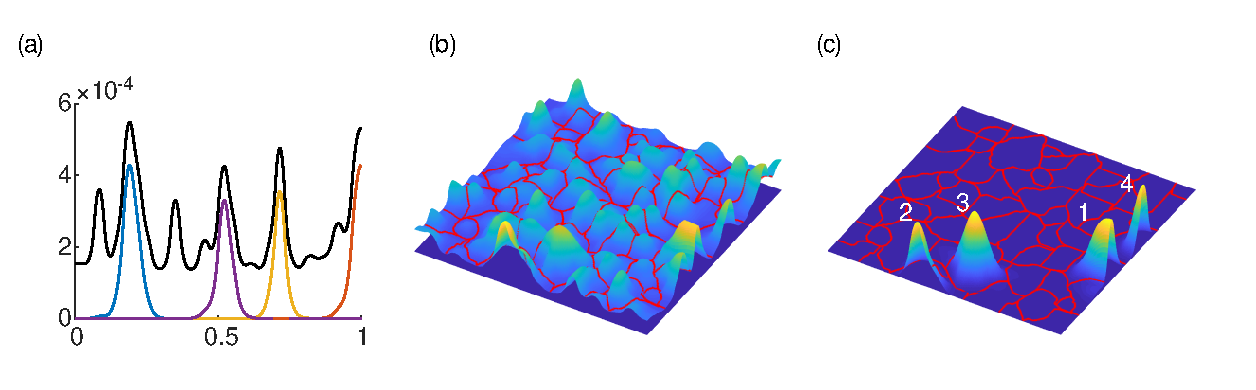
\includegraphics[width=\linewidth]{Fig1.eps}
\caption{(a) The landscape and first four eigenmodes obtained by simulating the system \eqref{eigenproblem} and \eqref{landscape} with Neumann boundary condition. The black line denotes the landscape and the colored lines are the eigenmodes. (b) The landscape and corresponding valley lines in a two-dimensional case. Red lines denote the valley lines. (c) The first four eigenmodes and corresponding valley lines, white numbers denote the rank of eigenmodes. Parameters are chosen as $K = 8000, N = 30$ for the one-dimensional case and $K = 8000, N = 20$ for the two-dimensional case. The potential $V$ is sampled from uniform distribution. }
\label{fig1}
\end{figure}

\subsection{Limit behavior}

Next, we focus on the limit behavior of the eigenmodes when the degree of randomness $K$ is very large. For simplicity, we assume that the potential function $V$ restricted to each sub-hypercube has the Bernoulli distribution \eqref{bernoulli}, which can only take the value of $0$ or $1$. Let
\begin{equation*}
D = \{x \in \Omega: V(x) = 0\}
\end{equation*}
denote the collection of sub-hypercubes at which the potential vanishes. We firstly consider the behavior of eigenmodes outside $D$. Let $x$ be the initial value of the reflecting diffusion $X_t$ solving the Skorokhod equation \eqref{reflecting}. When $x \notin D$, we have $V(X_s) = 1$ when $s$ is small, which implies that
\begin{equation*}
\int_{0}^{t} V(X_s) ds > 0, \quad \forall \; t > 0.
\end{equation*}
It thus follows from the probabilistic representation \eqref{probeigen} and the dominated convergence theorem that
\begin{equation}\label{largeK}
\lim_{K \rightarrow \infty} u(x) = 0, \quad \forall \; x \notin D.
\end{equation}
This shows that all eigenmodes must vanish outside $D$ in the limit of $K \rightarrow \infty$. In other words, when the degree of randomness $K$ is very large, the eigenmodes can only localize in the subdomain at which the potential attains its minimum. This means that the quantum states will converge to the position with the lowest potential energy.

We next focus on the behavior of eigenmodes inside $D$. Clearly, $D$ can be decomposed as the disjoint union of several connected components:
\begin{equation*}
D = D_1 \cup D_2 \cup \cdots \cup D_N.
\end{equation*}
In the limit of $K\rightarrow\infty$, since the potential vanishes in $D$, the eigenmode $u$ must satisfy the following local eigenvalue problem in each subdomain $D_k$:
\begin{equation}\label{subdomain}
\left\{
\begin{split}
& - L u = \lambda u \quad \textrm{in}\;\;\Omega, \\
& \quad g \frac{\partial u}{\partial n} + h u = 0 \quad \textrm{on}\;\;\partial D_k \cap \partial \Omega, \\
& \quad u = 0 \quad \textrm{on}\;\;\partial D_k \setminus \partial \Omega.
\end{split}
\right.
\end{equation}
Therefore, in the limit of $K \rightarrow \infty$, the spectrum of the Hamiltonian $H = - L + K V$ is composed of the local eigenvalues of the operator $-L$ in each subdomain $D_k$. If an eigenvalue of $H$ coincides with one of the local eigenvalues of $-L$ in $D_k$, then the corresponding eigenmode will be localized in $D_k$; conversely, if an eigenvalue of $H$ coincides with neither one of the local eigenvalues of $-L$ in $D_k$, then the corresponding eigenmode will not be localized in $D_k$. Based on the above discussion, if multiple subdomains $D_{k_1}, \cdots , D_{k_r}$ share a common local eigenvalue, then the corresponding eigenmode will have multiple peaks and the system will display \emph{multimodality}. In this case, there are more than one eigenvalue sharing a common value and the corresponding eigenmodes are composed of the local eigenmodes of subdomains.

Fig. \ref{fig2} (a) illustrates the potential, landscape and eigenmodes for a one-dimensional problem when $K$ is very large. It can be seen from the figure that the peaks of landscape and eigenmodes only appear on the subdomains in which $V = 0$. Fig. \ref{fig2} (b), (c) illustrates the potential and valley lines for a two-dimensional problem under different $K$. When $K$ is small, the subdomains predicted by the valley lines have no significant relationship with $V$. But for sufficient large $K$, the connected components $D_1, \cdots, D_k$ in which $V = 0$ are exactly separated by the valley lines. 

\begin{figure}
\centering
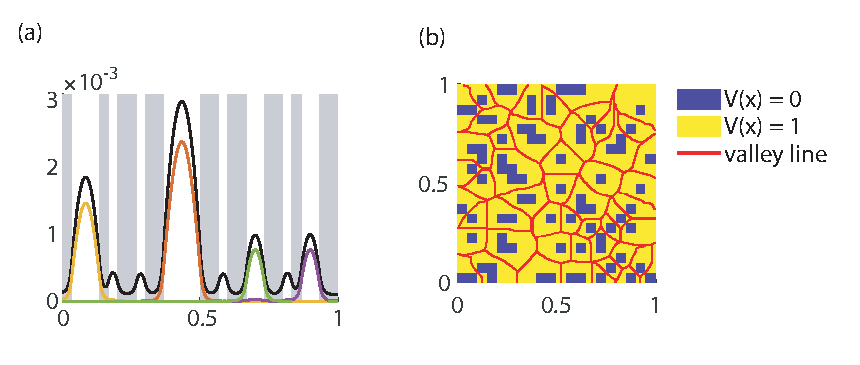
\includegraphics[width=\linewidth]{Fig2.eps}
\caption{(a) The potential, landscape and first four eigenmodes of a one-dimensional problem with Neumann boundary condition. The gray back ground denotes that $V = 1$ on the subdomain and the white background denotes $V = 0$. The black line denotes the landscape and the colored lines denote the eigenmodes. Parameters are chosen as $K = 10^4$ (b), (c) The potential and valley lines in a two-dimensional problem with Neumann boundary condition. The yellow parts denote that $V$ on the subdomains are $1$ and the blue parts denote $0$. Red lines denote the valley lines.}
\label{fig2}
\end{figure}

\section{Probability of localization to the boundary}\label{prob}

In the previous discussion, we develop our theory for the general model \eqref{eigenproblem} but in the following discussion, we only focus on the model \eqref{anderson}.

\subsection{Localization to the boundary}

As shown in Fig. \ref{fig1} (c), different with the Dirichlet boundary condition, eigenmodes of the problem with Neumann or Robin boundary condition may localize to the boundary. This means that only a part of the peak of these eigenmodes appears in the domain. When an eigenmode localize to the boundary, its boundary value may be very large. In this section, we will discuss the probability of the localization to the boundary. For simplicity, we only consider the first eigenmode.

For the one-dimensional case, for a certain eigenmode, the probability of its localization to the boundary is defined as
\begin{equation}
P_b = \frac{\max\{|u(0)|, |u(1)|\}}{\max_{x \in \Omega} |u(x)|},
\end{equation}
and for the two-dimensional case, we can define the probability of localization to the edge as
\begin{equation}
P_e = \frac{\max_{x \in \partial \Omega} |u(x)|}{\max_{x \in \Omega} |u(x)|},
\end{equation}
and the probability of localization to the corner is
\begin{equation}
P_c = \frac{\max\{|u(0,0)|, |u(0,1)|, |u(1,1)|, |u(1,0)|\}}{\max_{x \in \Omega} |u(x)|}.
\end{equation}

When the boundary condition of the problem is Dirichlet, $P_b$, $P_e$ and $P_c$ are constantly $0$. But for Robin and Neumann boundary condition, since the potential $V$ is randomly sampled from the Bernoulli distribution, $P_b$, $P_e$ and $P_c$ are random variables related to the parameter $p$, $K$ and $h$. Under such conditions, the probability of localization to the boundary, edge and corner under certain parameters are defined as the expectation of $P_b$, $P_e$ and $P_c$ respectively.

Fig. \ref{fig3} (a), (b) and (c) shows the variation of probability $P_b$, $P_e$ and $P_c$ with the parameter $h$, $p$ and $K$ for Robin boundary conditions respectively. Take the limit $h \rightarrow \infty$, then the boundary condition approaches Dirichlet and all the probability will decrease to $0$. The results shown in Fig. \ref{fig3} (a) are consistent with our discussion.

\subsection{Extended subdomains}

As shown in Section \ref{model}, for large $K$, the eigenmode localizes on the subdomain $D_k$ can be approximately regarded as solutions of the local eigenvalue problem \eqref{subdomain}. Furthermore, the first eigenmode of problem \eqref{anderson} should localize to the subdomain $D_k$ on which the local eigenvalue is the smallest in all connected branches of $D$. In the one-dimensional case, for Dirichlet boundary condition, the first eigenmode will localize to the longest subdomain. For Neumann boundary condition, the discussion of subdomains near the boundary becomes more complicated. We propose \emph{extended subdomain} to simplify the discussion with the help of symmetric properties.

Consider a Laplacian eigenvalue problem on an interval $D_k$ with left Neumann boundary condition and right Dirichlet boundary condition. Interval $D_k^{(e)}$ is twice as long as $D_k$. The Laplacian eigenvalue problem on $D_k^{(e)}$ has both side Dirichlet boundary condition. It's easy to prove that the smallest eigenvalue on $D$ is equal to the smallest eigenvalue on $D_k^{(e)}$. Furthermore, the first eigenmode on $D_k^{(e)}$ can be obtained from the first eigenmode on $D_k$ through mirror symmetry. Fig. \ref{fig3} (d) illustrates the first eigenmode on $D_k$ and $D_k^{(e)}$. We call the $D_k^{(e)}$ "extended subdomain".

Precisely, the extended subdomain can be defined as follows. For a problem with Neumann boundary condition, the extended subdomain $D_k^{(e)}$ is equal to $D_k$ when $D_k \cup \partial \Omega = \phi$. When $D_k \cup \partial \Omega \neq \phi$, all the extended subdomain $D_k^{(e)}$ can be obtained from $D_k$ through mirror symmetry along the boundary. In particular, in high-dimensional cases, when the subdomain is on the corner, the mirror symmetry will be done more than once. Fig. \ref{fig3} (e), (f) illustrate the potential and corresponding extended subdomains in the one-dimensional and two-dimensional case respectively.

With the help of the extended subdomain, we can transform all the local eigenvalue problems into Laplacian eigenvalue problems with Dirichlet boundary condition on extended subdomains. According to the discussions in Section \ref{model}, the first eigenmode of problem \eqref{anderson} will localize to the extended subdomain on which the Laplacian eigenvalue with Dirichlet boundary condition is the smallest. Especially, in the one-dimensional case, the first eigenmode will localize to the longest extended subdomain. If the longest two extended subdomains are same in length, the first eigenmode will display multimodality.

It can be seen in the figure that the extended subdomains on the boundary are more likely to have larger size and better symmetry, which cause the eigenmodes with Neumann boundary condition are more likely to localize to the boundary.

\begin{figure}
\centering
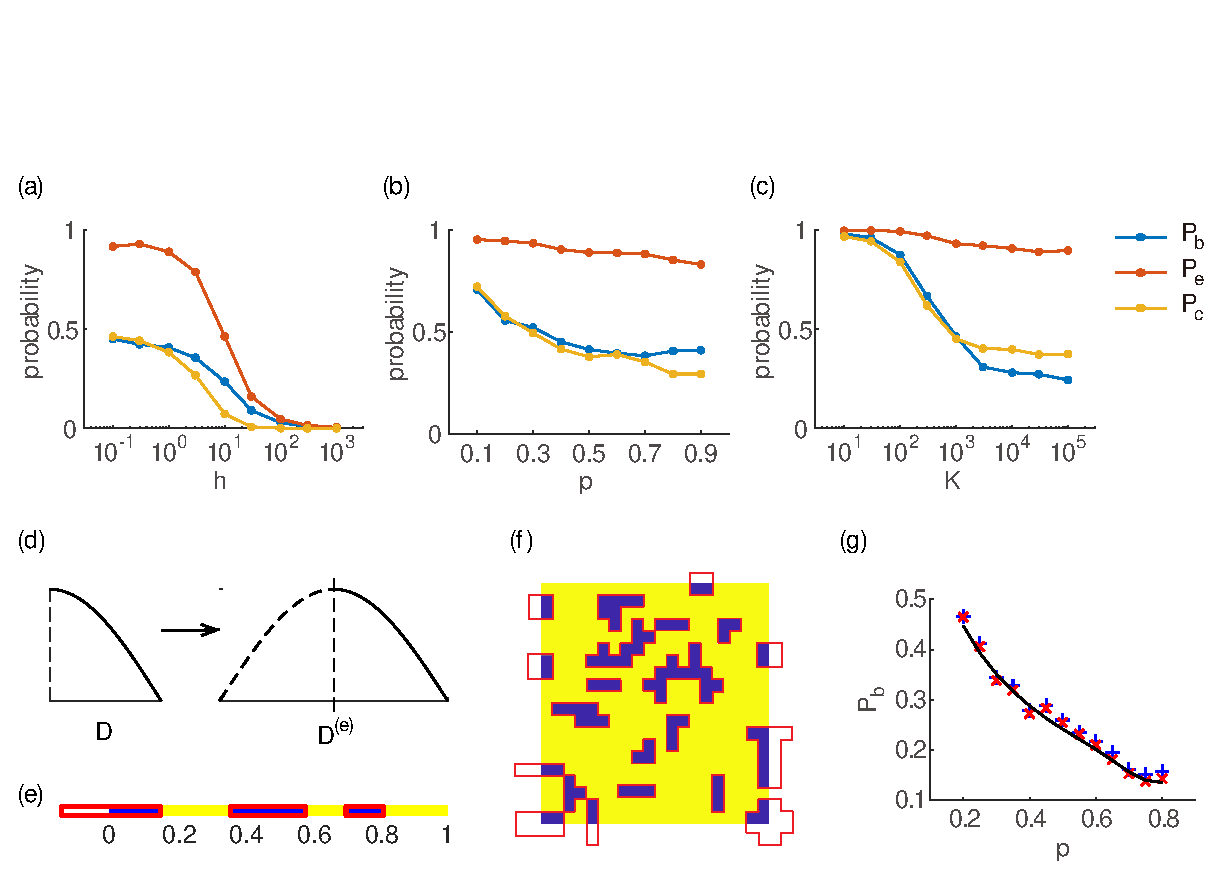
\includegraphics[width=\linewidth]{Fig3.eps}
\caption{(a), (b) and (c) Simulation results of the probability of localization to the boundary. Default parameters are chosen as $K = 10^3, h = 1, p = 0.5$ if not mentioned. For the one-dimensional case, the whole domain is divided into $N = 50$ intervals and for the two-dimensional case, we choose $N = 50$. (d) The first eigenmode of the Laplacian eigenvalue problem on $D$ and $D^{(e)}$. (e), (f) The potential and extended subdomains in one-dimensional and two-dimensional case respectively. Blue parts denote subdomains on which $V = 0$ and yellow parts denote $V = 1$. Extended subdomains $D^{(e)}$ are surrounded by red lines. (g) Simulation results and theoretical predictions of the probability of localization to the boundary for the one-dimensional case. Blue crosses denote the simulation result of the probability $P_b$ for different parameter $p$, red crosses denote the frequency of the event "the longest extended subdomain locates on the boundary" in the simulation and the black line denotes the theoretical prediction of $P_b$ from equation \eqref{bdprob}. Parameters are chosen as $K = 5 \times 10^4, h = 0.01, N = 50$. We randomly generate the potential $1000$ times on each point and calculate the mean value of the samples as the results of the probability.}
\label{fig3}
\end{figure}

\subsection{A theoretical result for the one-dimensional case}

In the one-dimensional case, the whole domain $[0, 1]$ is divided uniformly into $N$ intervals. In each interval, the potential $V$ is constant with its value being sampled from the Bernoulli distribution. The values of the potential in different intervals are independent to each other.

Suppose that the previous two intervals on which $V$ takes the value $1$ and $0$ respectively. Then the number of following intervals on which $V$ takes the value $0$ is a random variable $X$. $X$ takes the value $n$ means that the values of $V$ on the next $n-1$ intervals are $0$ and the value on the next $n$-th is $1$. For a sufficient large $N$, the random variable $X$ approximately obeys the geometric distribution with parameter $p$. This means that
$$ \mathbb{P}(X = n) = q^{n-1} p, $$
where $q = 1 - p$.

Similarly, the number of continuous intervals on which $V$ takes the value $1$ is also a random variable $Y$ with distribution
$$ \mathbb{P}(Y = n) = p^{n-1} q. $$

In the whole domain $[0, 1]$, subdomains on which $V = 0$ and $V = 1$ must appear alternately. Two adjacent subdomains are called a \emph{period}. The average length of each period is $\Enum(X + Y) = \frac{1}{p q}$. Therefore, the average number of periods in the whole domain is $M = N p q$. We can approximately assume that the whole domain consists of subdomains taking values $0$ and $1$ alternately with length $X_1, Y_1, \cdots, X_M, Y_M$. For a sufficient large $N$, the random variables $X_1, Y_1, \cdots, X_M, Y_M$ are approximately independent.

For a sufficient big $K$ and a sufficient small $h$, the probability of that the first eigenmode localize to the boundary is equal to the probability of the event that the longest extended subdomain locates on the boundary. We can obtain its probability is
\begin{equation}\label{bdprob}
P_b = q^2 p^2 \sum_{k=1}^{\infty} q^{k-2} \sum_{n=1}^{k-1} (1 - q^{2 \max\{k-n,n\}-1})^{M-2} + p q^2 \sum_{n=1}^{\infty} (1 - p^{2 n-1})^{M-2} p^{n-1}.
\end{equation}
Detailed calculations are given in Appendix \ref{AppendixB1}.

Fig. \ref{fig3} (g) illustrates the simulation results and theoretical predictions. The theoretical prediction is in good agreement with the simulation.

\begin{remark}
Here we choose the parameter $h$ to be small but not $0$ to avoid the multimodality in Fig. \ref{fig3}. Under such conditions, if the longest two extended subdomains have the same length but only one of them locates on the boundary, then the first eigenmode will not localize to the boundary. This can help us to avoid some complicated discussions.
\end{remark}

\section{Multimodality}\label{multimodality}

As shown before, the first eigenmode will localize to the extended subdomain on which the local eigenvalue is the smallest. If multiple subdomains share a common local eigenvalue, then the corresponding eigenmodes will have multiple peaks and all the corresponding eigenvalues are equal, which is called \emph{multimodality}. That is to say, the first eigenmode appears multimodality is equivalent to that the first and the second eigenvalue are equal. Fig. \ref{fig4} (a) illustrates an example of multimodality. For simplicity, we only focus on the multimodality of the first eigenmode in the one-dimensional case. For the one-dimensional case, the first eigenmode will localize to the longest extended subdomain. When there are more than one longest extended subdomains, the multimodality occurs on the first eigenmode.

The probability of that the first eigenmode appears multimodality is equal to the probability of that there are more than one longest extended subdomains. For simplicity, we only consider the longest two subdomains.

For Dirichlet boundary condition, we can obtain the probability of multimodality is
\begin{equation}\label{multiD}
P_D = 1 - p \sum_{n=1}^{\infty} (1 - p^{n-1})^{M-2} q^{n-1},
\end{equation}
and for Neumann boundary condition, probability of multimodality is
\begin{equation}\label{multiN}
\begin{split}
P_N = 1 - & q^2 (M-2) \sum_{n=1}^{\infty} (1 - q^{(n-1)/2})^2 (1 - q^{n-1})^{M-3} q^{n-1} p \\
- & 2 q^2 \sum_{n=1}^{\infty} (1 - q^{2n-1})^{M-2} (1 - q^{n-1}) q^{n-1} p \\
- & 2 p q (M-1) \sum_{n=1}^{\infty} (1 - q^{(n-1)/2}) (1 - q^{n-1})^{M-2} q^{n-1} p \\
- & 2 p q \sum_{n=1}^{\infty} (1 - q^{2n-1})^{M-1} q^{n-1} p \\
- & p^2 M \sum_{n=1}^{\infty} (1 - p^{n-1})^{M-1} q^{n-1} p.
\end{split}
\end{equation}
Detailed calculations are given in Appendix \ref{AppendixB2} and Appendix \ref{AppendixB3}.

Affected by calculation error, we can hardly observe that eigenvalues are exactly equal in practice. We regard that the multimodality appears when the relative difference between the first and the second eigenvalue satisfy $\frac{\lambda_2 - \lambda_1}{\lambda_1} < 0.02$. Fig. \ref{fig4} (b), (c) illustrate the simulation results and theoretical predictions for both Dirichlet and Neumann boundary condition. The theoretical prediction is in good agreement with the simulation.

\begin{figure}
\centering
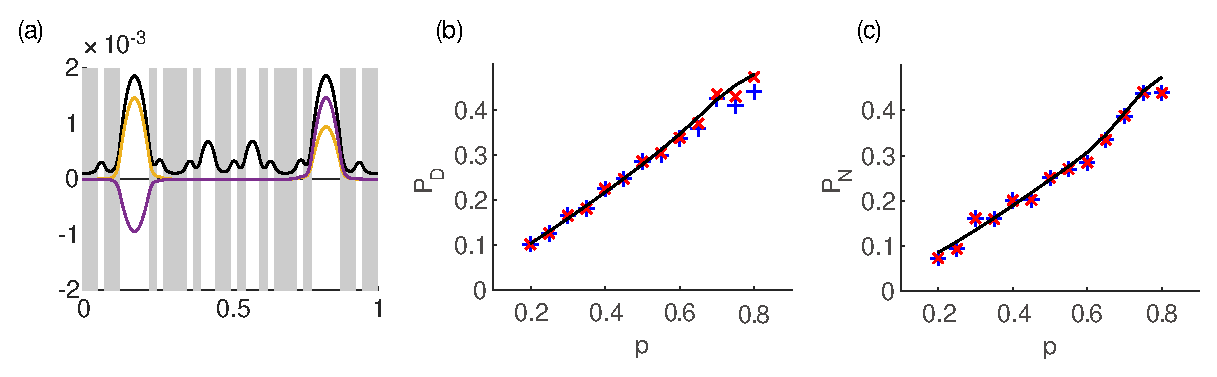
\includegraphics[width=\linewidth]{Fig4.eps}
\caption{(a) A one-dimensional example of multimodality with the Neumann boundary condition. The gray background denotes $V = 1$ on the subdomain and the white background denotes $0$. The black line denotes the landscape and the colored lines denote the eigenmodes.  Parameter is chosen as $K = 10^4$. In this example, the first and the second eigenvalue are both $\lambda_1 = \lambda_2 = 681.5523$. (b), (c) Simulation results and theoretical predictions of the probability of multimodality under Dirichlet and Neumann boundary condition respectively. Blue crosses denote the frequency of multimodality for different parameter $p$, red crosses denote the frequency of the event that there are more than one longest extended subdomains and the black line denotes the theoretical prediction of $P_D$ and $P_N$ obtained from equation \eqref{multiD} and \eqref{multiN}. Parameters are chosen as $K = 3 \times 10^6, N = 50$. We randomly generate the potential $1000$ times on each point and calculate the mean value of the samples as the results of the probability.}
\label{fig4}
\end{figure}

\section{Phase transition}\label{phase}

\subsection{Model of the phase transition}

Consider a one-dimensional problem with parabolic boundary condition. The potential $V$ is chosen as follows. As shown in Fig. \ref{fig5} (a), in the whole domain $[0,1]$, the values of $V$ are $0$ and $1$ alternately in these intervals with length $L_2/2, L_1, L_2, L_3, L_4, L_3, L_2/2$ respectively.
\begin{equation}
V = \left\{
\begin{split}
1 & \quad x \in [0, x_1), \\
0 & \quad x \in [x_1, x_2), \\
1 & \quad x \in [x_2, x_3), \\
0 & \quad x \in [x_3, x_4), \\
1 & \quad x \in [x_4, x_5), \\
0 & \quad x \in [x_5, x_6), \\
1 & \quad x \in [x_6, 1].
\end{split}
\right.
\end{equation}
where
\begin{equation}
\begin{split}
x_1 = L_2/2, \quad x_2 = L_2/2 + L_1, \quad x_3 = L_2/2 + L_1 + L_2, \quad x_4 = L_2/2 + L_1 + L_2 + L_3, \\
x_5 = L_2/2 + L_1 + L_2 + L_3 + L_4, \quad x_6 = L_2/2 + L_1 + L_2 + L_3 + L_4 + L_3.
\end{split}
\end{equation}
The potential can be viewed as two wells $W_1$ and $W_2$ with length $L_1$ and $2 L_3$ while there is a barrier with length $L_4$ in the middle of the second well. The phase transition problem can be described as
\begin{equation}
S: \;
\left\{
\begin{split}
& -\triangle u + K V u = \lambda u, \quad \textrm{in} \; (0, 1), \\
& u(0) = u(1), \quad u'(0) =  u'(1).
\end{split}
\right.
\end{equation}

In the phase transition problem, $L_2$ is big enough to separate two wells and the length of barrier $L_4$ is small. For details, the parameters should satisfy: $L_3 < L_1 < 2 L_3$ (two wells should be approximately same in length), $L_4 < L_3 / 2$ (barrier should be short enough), $L_2 > L_1+ L_3 + L_4 + L_3$ ($L_2$ should be big enough to separate the two wells), and the total length $L_1 + 2 L_2 + 2L_3 + L_4 = 1$.

The first eigenmode and the second eigenmode of the problem for different $K$ are illustrated in Fig. \ref{fig5} (b). Since the second well $W_2$ is longer, when $K$ is small, the barrier in $W_2$ is not strong enough, then the first eigenmode will localize to $W_2$. On the contrary, when $K$ is big, the first eigenmode will localize to $W_1$. As the parameter $K$ increasing, the left peak of the first eigenmode becomes higher and the right peak vanishes. Then the location of the maxima of the first eigenmode will jump from $W_2$ to $W_1$, which is called \emph{phase transition}. Due to the orthogonality, the behavior of the second eigenmode is the opposite of the first, location of the maxima of the second eigenmode will jump from $W_1$ to $W_2$.

For details, we define the relative height of the left peak of eigenmode $u$ as 
\begin{equation}
F = \frac{\max_{x \in W_1} |u(x)|}{\max_{x \in W_1} |u(x)| + \max_{x \in W_2} |u(x)|}.
\end{equation}
In a certain range, it's obvious that the relative height $F$ of the first eigenmode increases with $K$. Fig. \ref{fig5} (c) illustrates the variation of the relative height $F$ of the first eigenmode with the parameter $K$. There exists a value of $K$ satisfy the left peak and the right peak of $u_1$ are equal in height, that is $F = 0.5$. The parameter $K$ which satisfy $F = 0.5$ is defined as the \emph{critical point} $K_c$ in phase transition.

\subsection{System decomposition}

In the phase transition problem, the potential has two wells. The two wells are so far apart that we can approximately assume that they have no influence on each other. Thus, we can divide the problem $S$ into two subsystems $S_1, S_2$ and discuss the eigenmode localize to $W_1$ and $W_2$ separately. As shown in Fig. \ref{fig5} (a), set the value of $V(x)$ in $W_1$ to $1$ and we can obtain $V_2(x)$. Similarly, set the value in $W_2$ to $1$ and we can obtain $V_1(x)$.
\begin{equation}
V_1 = \left\{
\begin{split}
1 & \quad x \in [0, x_1), \\
0 & \quad x \in [x_1, x_2), \\
1 & \quad x \in [x_2, 1].
\end{split}
\right.
\qquad
\text{and}
\qquad
V_2 = \left\{
\begin{split}
1 & \quad x \in [0, x_3), \\
0 & \quad x \in [x_3, x_4), \\
1 & \quad x \in [x_4, x_5), \\
0 & \quad x \in [x_5, x_6), \\
1 & \quad x \in [x_6, 1].
\end{split}
\right.
\end{equation}
The original system $S$ can be decomposed into two subsystems $S_1$ and $S_2$ with potential $V_1(x)$ and $V_2(x)$ separately.
\begin{equation}
S_i: \;
\left\{
\begin{split}
& -\triangle u + K V_i u = \lambda u, \quad \textrm{in} \; (0, 1), \\
& u(0) = u(1), \quad u'(0) =  u'(1).
\end{split}
\right.
\quad
i = 1, 2.
\end{equation}
For the first two eigenmodes, the eigenmode localized to $W_1$ corresponds to subsystem $S_1$, and the other eigenmode corresponds to subsystem $S_2$. 

Fig. \ref{fig5} (d) illustrates the first two eigenmodes of the original system $S$ and the first eigenmode of two subsystems. It can be seen from the figure that the eigenmode of each subsystem are almost the same as the eigenmode of the original system in the corresponding well. Fig. \ref{fig5} (e) illustrates the eigenvalues of the original system and subsystems for different $K$. The eigenvalues of the subsystems are good approximations to the eigenvalues of the original system.

Now we can give some detailed explanation of the phase transition problem. The eigenvalue of each subsystem increases with the increasing of $K$, but eigenvalues of both subsystems increase at different rates. When $K$ is small, the eigenvalue of $S_2$ is smaller, then the subsystem $S_2$ is dominant, the first eigenmode of $S$ will localize to $W_2$. As the parameter $K$ increasing, eigenvalue of $S_1$ will exceed the eigenvalue of $S_2$, then the minimum eigenvalue changes from one to the other. At that time, the localization of the first eigenmode will change from $W_2$ to $W_1$, which means that the phase transition occurs. Similar to the multimodality, the phase transition occurs when the first and the second eigenvalues of the original system $S$ are equal. This means that the first eigenvalues of both subsystems are equal. The value of the eigenvalue when phase transition occur is defined as the critical eigenvalue $\lambda_c$.

\begin{figure}
\centering
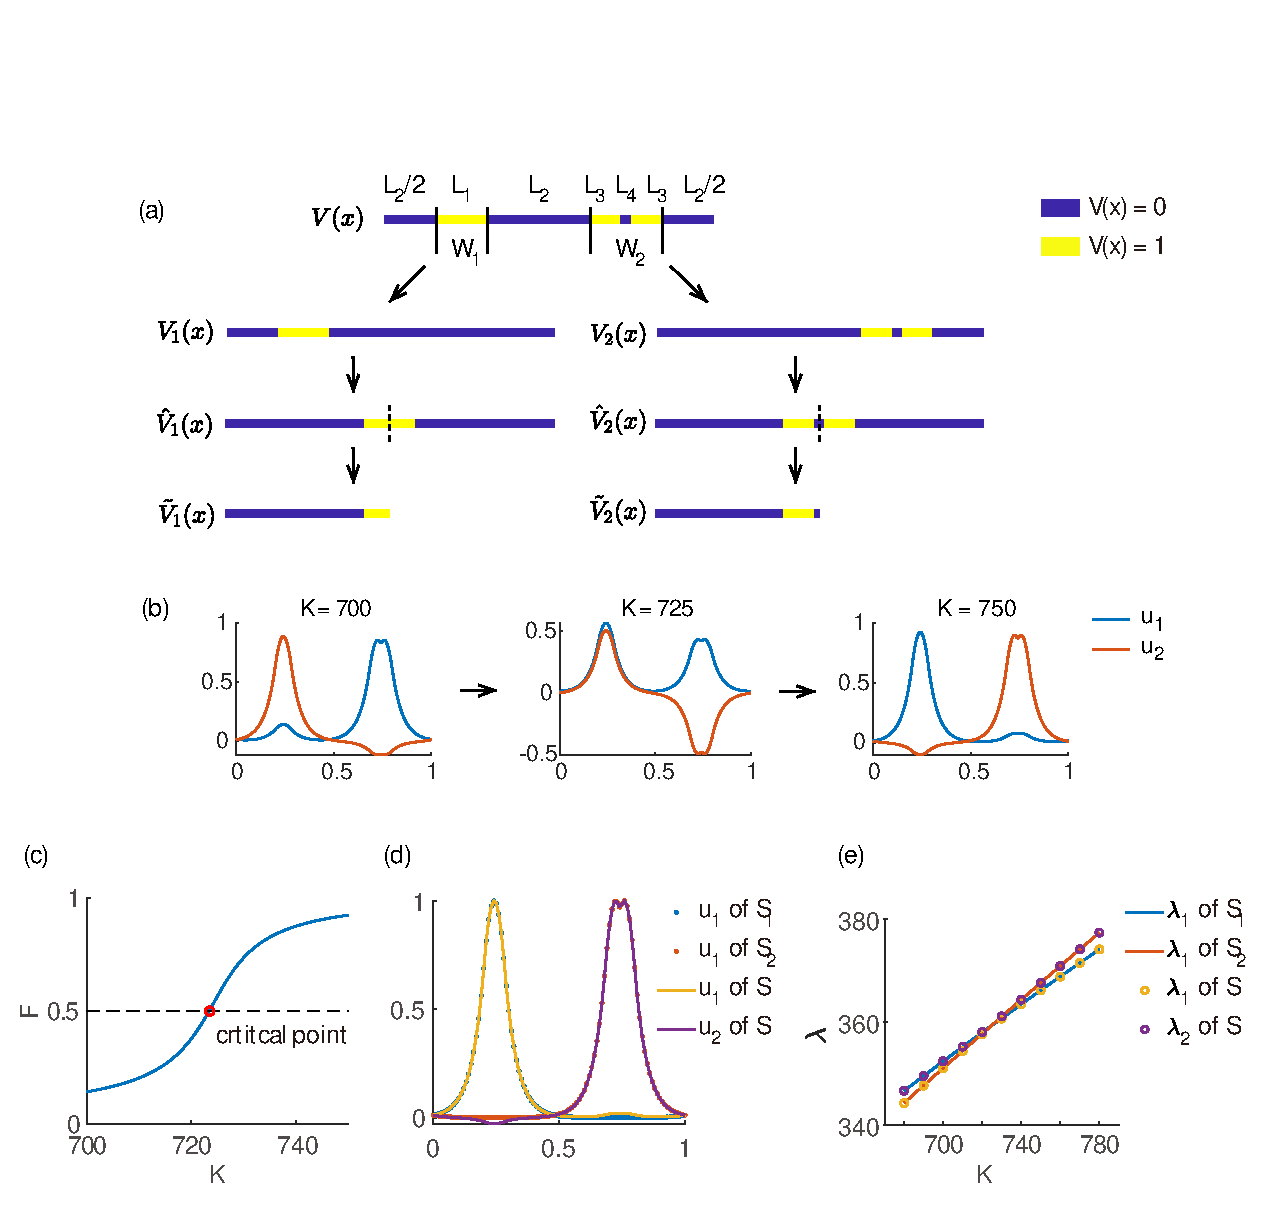
\includegraphics[width=\linewidth]{Fig5.eps}
\caption{(a) Potentials mentioned in the phase transition problem. Blue parts denote subdomains on which $V = 0$ and yellow parts denote $V = 1$. (b) The first eigenmode $u_1$ and the second eigenmode $u_2$ for different $K$ in the phase transition problem. (c) The relative height $F$ of the first eigenmode $u_1$ for different $K$. The black dotted line denotes the line $F = 0.5$ and the red circle denotes the critical point. (d), (e) Eigenmodes and eigenvalues of the original system $S$ and two subsystems $S_1$ and $S_2$ respectively. We choose the parameter $K = 800$ in (d). Parameters are chosen as $L_1 = 1/12, L_2 = 2/5, L_3= 1/20, L_4 = 1/60$ in all figures.}
\label{fig5}
\end{figure}

\subsection{Eigenvalue of the subsystems}

Consider the subsystem $S_1$, thanks to the periodicity, we can shift the potential freely. As shown in \ref{fig5} (a), we can move the well $W_1$ to the middle of the whole interval without changing the eigenvalues of the subsystem. We can easily prove that eigenvalues of subsystem $S_1$ is equal to the eigenvalues of a system $\hat{S}_1$ with the potential $\hat{V}_1$. The potential $\hat{V}_1$ is defined as
\begin{equation}
\hat{V}_1 = \left\{
\begin{split}
1 & \quad x \in [0, \frac{1 - L_1}{2}), \\
0 & \quad x \in [\frac{1 - L_1}{2}, \frac{1 + L_1}{2}), \\
1 & \quad x \in [\frac{1 + L_1}{2}, 1).
\end{split}
\right.
\end{equation}
Similarly, we can define
\begin{equation}
\hat{V}_2 = \left\{
\begin{split}
1 & \quad x \in [0, \frac{1 - L_4 - 2 L_3}{2}), \\
0 & \quad x \in [\frac{1 - L_4 - 2 L_3}{2}, \frac{1 - L_4}{2}), \\
1 & \quad x \in [\frac{1 - L_4}{2}, \frac{1 + L_4}{2}), \\
0 & \quad x \in [\frac{1 + L_4}{2}, \frac{1 + L_4 + 2 L_3}{2}), \\
1 & \quad x \in [\frac{1 + L_4 + 2 L_3}{2}, 1].
\end{split}
\right.
\end{equation}

Due to the symmetry, noting that both potential $\hat{V}_i$ satisfy $\hat{V}_i(x) = \hat{V}_i(1-x)$, then the eigenmodes of $\hat{S}_i$ should also satisfy $u(x) = u(1-x)$. We can prove that eigenmodes of the subsystem should satisfy $u'(0) = u'(1/2) = 0$. The eigenvalues of the system are equal to the eigenvalues of a problem defined on interval $[0, 1/2]$ with Neumann boundary condition, whose potential $\tilde{V}_1$ is defined as
\begin{equation}
\tilde{V}_i(x) = \hat{V}_i(x) \qquad x \in [0, 1/2], \quad i = 1, 2.
\end{equation}
\begin{equation}
\tilde{S}_i: \;
\left\{
\begin{split}
& -\triangle u + K \tilde{V}_i u = \lambda u, \quad \textrm{in} \; (0, 1/2), \\
& u'(0) = u'(1/2) = 0
\end{split}
\right.
\quad
i = 1, 2.
\end{equation}
It is easy to prove that the eigenvalues of the subsystems $S_1$ and $S_2$ are equal to the eigenvalues of $\tilde{S}_1$ and $\tilde{S}_2$ respectively. The potentials $\tilde{V}_1$ and $\tilde{V}_2$ are also shown in Fig. \ref{fig5} (a).

After simplified, for certain $K$, each eigenvalue $\lambda$ of subsystem $S_1$ satisfy the equation
\begin{equation}\label{phase1}
0 = D_1(K, \lambda) = \alpha \tan(\alpha t_0) - \beta \tanh(\beta (\frac12 - t_0)),
\end{equation}
where $\alpha = \sqrt{\lambda}, \beta = \sqrt{K - \lambda}, t_0 = L_1 / 2$.

Similarly, the first eigenvalue of subsystem $S_2$ satisfy the equation
\begin{equation}\label{phase2}
\begin{split}
0 = D_2(K, \lambda) = & (\alpha^2 - \beta^2)(\mathrm{e}^{2 \beta t_2} + \mathrm{e}^{2 \beta (t_1+t_3)}) / (\mathrm{e}^{2 \beta (t_1+t_3)} - \mathrm{e}^{2 \beta t_2}) \\
& + (\alpha^2 + \beta^2)(\mathrm{e}^{2 \beta t_3} + \mathrm{e}^{2 \beta (t_1+t_2)}) / (\mathrm{e}^{2 \beta (t_1+t_3)} - \mathrm{e}^{2 \beta t_2}) \\
& + 2 \alpha \beta \cot(\alpha (t_1 - t_2))
\end{split},
\end{equation}
where $t_1 = L_4 / 2, t_2 = L_4 / 2 + L_3, t_3 = 1 / 2$. Detailed calculations are given in Appendix \ref{AppendixC}.

When phase transition occurs, the first eigenvalues of the both subsystems are equal. Then the critical point $K_c$ and the critical eigenvalue $\lambda_c$ satisfy
\begin{equation}\label{phase0}
\left\{
\begin{split}
D_1(K_c, \lambda_c) = 0 \\
D_2(K_c, \lambda_c) = 0
\end{split}
\right.
\end{equation}
Basing the equation \eqref{phase0}, we can predict the critical point and the critical eigenvalue of the problem.

We generate $L_1, L_2, L_3, L_4$ randomly as our sample points. The sample points satisfy $0.03 < L_3 < 0.055$, $1.3 L_3 < L_1 < 1.7 L_3$, $0.2 L_3 < L_4 < 0.4 L_3$ and $L_1 + 2 L_2 + 2 L_3 + L_4 = 1$. On $1000$ sample points, mean square error (MSE) of the critical point $K_c$ is $0.3947$, and MSE of the critical eigenvalue $\lambda_c$ is $9.1751$. The predicted values obtained from \eqref{phase0} are very close to the simulation results.

\begin{remark}
Noting that there are two descriptions of the critical point $K_c$ mentioned above. One is that two peaks of the first eigenmode locates in $W_1$ and $W_2$ are equal in height ($F = 0.5$) and the other is that the first and the second eigenvalues of the original system are equal ($\lambda_1 = \lambda_2$). Actually, the two descriptions are not exactly same, which is the main source of the error mentioned above. The simulation results prove that the difference between two descriptions is sufficient small.
\end{remark}

\section*{Acknowledgements}
The authors acknowledge support from the NSAF grant in National Natural Science Foundation of China (NSFC) with grant No. U1930402.

\setlength{\bibsep}{5pt}
\small\bibliographystyle{nature}
\bibliography{localization}


\begin{appendices}

\section{Proof of the Filochea-Mayboroda inequality}\label{AppendixA}

Let $(X, F)$ be the solution to the Skorokhod stochastic differential equation
\begin{equation*}
d X_t = b(X_t) dt + \sigma(X_t) d W_t - g(X_t) n(X_t) d F_t,
\end{equation*}
where $F$ is a continuous increasing process that increases when $X_t \in \partial \Omega$. For convenience, let
\begin{equation*}
Y_t = e^{\int_{0}^{t} h(X_s) d F_s - \int_{0}^{t} K V(X_s) ds}.
\end{equation*}
By Ito's formula, we have
\begin{equation*}
\begin{split}
du(X_t) Y_t = & u(X_t) Y_t [h(X_t) dF_t - K V(X_t) dt] + \partial_i u(X_t) Y_t dX^i_t + \frac{1}{2} \partial_{ij} u(X_t) Y_t (dX^i_t) (dX^j_t) \\
= & u(X_t) Y_t [h(X_t) dF_t - K V(X_t) dt] + \partial_i u(X_t) b^i(X_t) Y_t dt + \partial_i u(X_t) \sigma^i_j(X_t) Y_t dW^j_t \\
& + \partial_i u(X_t) g(X_t) n^i(X_t) Y_t dF_t + \frac{1}{2} \partial_{ij} u(X_t) a^{ij}(X_t) Y_t dt\\
= & \partial_i u(X_t) \sigma^i_j(X_t) Y_t dW^j_t + (L u - K V u) (X_t) Y_t dt
+\left( g \frac{\partial u}{\partial n} + h u \right) (X_t) Y_t dF_t,
\end{split}
\end{equation*}
where we have used Einstein's summation convention: if the same index appears twice in any term, once as an upper index and once as a lower index, that term is understood to be summed over all possible values of that index. Since $F_t$ only increases when $X_t \in \partial \Omega$ and since $g \partial u/\partial n + h u = 0$ on $\partial \Omega$, we obtain
\begin{equation*}
du(X_t) Y_t = \partial_i u(X_t) \sigma^i_j(X_t) Y_t dW^j_t - \lambda u(X_t) Y_tdt.
\end{equation*}
This shows that
\begin{equation*}
u(X_t)Y_t = u(X_0) + \int_0^t \partial_i u(X_s) \sigma^i_j(X_s) Y_s dW^j_s - \lambda \int_0^t u(X_s) Y_s ds.
\end{equation*}
Thus we have
\begin{equation*}
u(x) = \Enum_xu(X_t)Y_t+\lambda\Enum_x\int_0^t u(X_s)Y_sds.
\end{equation*}
Taking $t\rightarrow\infty$ in the above equation yields
\begin{equation*}
u(x) = \lambda\Enum_x\int_0^\infty u(X_s)Y_sds.
\end{equation*}
Recall that the localization landscape $w = w(x)$ is defined as the solution to the following PDE:
\begin{equation*}
\left\{
\begin{split}
& - L w + K V w = 1 \quad \textrm{in} \; \Omega, \\
& \quad g \frac{\partial w}{\partial n} + h w = 0 \quad \textrm{on} \; \partial \Omega,
\end{split}\right.
\end{equation*}
Similarly, the landscape has the following probabilistic representation:
\begin{equation*}
w(x) = \Enum_x\int_0^\infty Y_sds.
\end{equation*}

\section{Geometry distribution approximation}\label{AppendixB}

Let random variables $X_1, Y_1, \cdots, X_M, Y_M$ are independent, with distribution
$$ \mathbb{P}(X_k = n) = q^{n-1} p \quad \mathbb{P}(Y_k = n) = p^{n-1} q \qquad k = 1, 2, \cdots, M, $$
thus
$$ \mathbb{P}(X_k < n) = 1 - q^{n-1}, $$
where $q = 1 - p$ and $M = N p q$.

\subsection{Calculation of \eqref{bdprob}}\label{AppendixB1}

For Neumann boundary conditions, event "the longest extended subdomain appears on the boundary" can be divided into the following situations:

\paragraph*{situation 1}
$V(0) = V(1) = 0$ with probability $q^2$. Under such conditions, length of extended subdomains are $2 X_1, X_2, \cdots, X_{M-1}, 2 X_M$.

Then we have
\begin{equation*}
\begin{split}
  & \mathbb{P}(\text{the longest extended subdomain appears on the boundary}) \\
= & \mathbb{P}(\max\{X_2, X_3, \cdots, X_{M-1}\} < 2 \max\{X_1, X_M\}) \\
= & \sum_{m,n=1}^{\infty} \mathbb{P}(\max\{X_2, X_3, \cdots, X_{M-1}\} < 2 \max\{m,  n\}) \mathbb{P}(X_1 = m) \mathbb{P}(X_M = n) \\
= & \sum_{m,n=1}^{\infty} [\mathbb{P}(X_k < 2 \max\{m,n\}) ]^{M-2} \mathbb{P}(X_1 = m) \mathbb{P}(X_M = n)\\
= & \sum_{m,n=1}^{\infty} (1 - q^{2 \max\{m,n\}-1})^{M-2} q^{m-1} p q^{n-1} p\\
= & \sum_{k=1}^{\infty} q^{k-2} p^2 \sum_{n=1}^{k-1} (1 - q^{2 \max\{k-n,n\}-1})^{M-2} 
\end{split}.
\end{equation*}

\paragraph*{situation 2}
$V(0) = 0, V(1) = 1$ with probability $p q$. Under such conditions, length of extended subdomains are $2 X_1, X_2, \cdots, X_M$.

Then we have
\begin{equation*}
\begin{split}
  & \mathbb{P}(\text{the longest extended subdomain appears on the boundary}) \\
= & \mathbb{P}(\max\{X_2, X_3, \cdots, X_{M}\} < 2 X_1) \\
= & \sum_{n=1}^{\infty} \mathbb{P}(\max\{X_2, X_3, \cdots, X_{M-1}\} < 2 n) \mathbb{P}(X_1 = n) \\
= & \sum_{n=1}^{\infty} [\mathbb{P}(X_k < 2 n)]^{M-1} \mathbb{P}(X_1 = n)\\
= & q \sum_{n=1}^{\infty} (1 - p^{2 n-1})^{M-2} p^{n-1}
\end{split}.
\end{equation*}

\paragraph*{situation 3}
$V(0) = 1, V(1) = 0$ with probability $p q$. Under such conditions, length of extended subdomains are $2 X_1, X_2, \cdots, X_M$. It can be calculated similarly to situation 2.

In summary, probability of localize to the boundary is
\begin{equation*}
P_b = q^2 p^2 \sum_{k=1}^{\infty} q^{k-2} \sum_{n=1}^{k-1} (1 - q^{2 \max\{k-n,n\}-1})^{M-2} + p q^2 \sum_{n=1}^{\infty} (1 - p^{2 n-1})^{M-2} p^{n-1}.
\end{equation*}

\subsection{Calculation of \eqref{multiD}}\label{AppendixB2}

For Dirichlet Boundary, we have
\begin{equation*}
\begin{split}
P_D = & \mathbb{P}(\text{there is a unique longest subdomain}) \\
= & \sum_{k=1}^{M} \mathbb{P}(\max\{X_1, X_2, \cdots, X_{k-1}, X_{k+1}, \cdots, X_{M}\} < X_k) \\
= & M \; \mathbb{P}(\max\{X_{2}, X_{3}, \cdots, X_{M}\} < X_1) \\
= & M \sum_{n=1}^{\infty} \mathbb{P}(\max\{X_2, X_3, \cdots, X_{M-1}\} < n) \mathbb{P}(X_1 = n) \\
= & M \sum_{n=1}^{\infty} [\mathbb{P}(X_k < n)]^{M-1} \mathbb{P}(X_1 = n)\\
= & M \sum_{n=1}^{\infty} (1 - p^{n-1})^{M-1} q^{n-1} p
\end{split}.
\end{equation*}

\subsection{Calculation of \eqref{multiN}}\label{AppendixB3}

For Neumann Boundary, probability of "there is a unique longest extended subdomain" can be divided into the following situations:

\paragraph*{situation 1}
$V(0) = V(1) = 0$ with probability $q^2$. We have
\begin{equation*}
\begin{split}
  & \mathbb{P}(\text{there is a unique longest subdomain}) \\
= & \sum_{k=2}^{M-1} \mathbb{P}(\max\{2 X_1, X_2, \cdots, X_{k-1}, X_{k+1}, \cdots, 2 X_{M}\} < X_k) \\
& + \mathbb{P}(\max\{X_2, \cdots, X_{M-1}, 2 X_M\} < 2 X_1) \\
& + \mathbb{P}(\max\{2 X_1, X_2, \cdots, X_{M-1}\} < 2 X_M) \\
= & (M-2) \mathbb{P}(\max\{2 X_1, X_3 \cdots, 2 X_{M}\} < X_2) \\
& + 2 \mathbb{P}(\max\{X_2, \cdots, X_{M-1}, 2 X_M\} < 2 X_1) \\
= & (M-2) \sum_{n=1}^{\infty} \mathbb{P}(\max\{2 X_1, X_3 \cdots, 2 X_{M}\} < n) \mathbb{P}(X_2 = n) \\
& + 2 \sum_{n=1}^{\infty} \mathbb{P}(\max\{X_2, \cdots, X_{M-1}, 2 X_M\} < 2 n) \mathbb{P}(X_1 = n) \\
= & (M-2) \sum_{n=1}^{\infty} [\mathbb{P}(2 X_k < n)]^2 [\mathbb{P}(X_k < n)]^{M-3} \mathbb{P}(X_2 = n) \\
& + 2 \sum_{n=1}^{\infty} [\mathbb{P}(X_k < 2 n)]^{M-2} \mathbb{P}(X_k < n) \mathbb{P}(X_1 = n) \\
= & (M-2) \sum_{n=1}^{\infty} (1 - q^{(n-1)/2})^2 (1 - q^{n-1})^{M-3} q^{n-1} p \\
& + 2 \sum_{n=1}^{\infty} (1 - q^{2n-1})^{M-2} (1 - q^{n-1}) q^{n-1} p
\end{split}.
\end{equation*}

\paragraph*{situation 2}
$V(0) = 0, V(1) = 1$ with probability $p q$. We have
\begin{equation*}
\begin{split}
  & \mathbb{P}(\text{there is a unique longest subdomain}) \\
= & \sum_{k=2}^{M} \mathbb{P}(\max\{2 X_1, X_2, \cdots, X_{k-1}, X_{k+1}, \cdots, X_{M}\} < X_k) \\
& + \mathbb{P}(\max\{X_2, \cdots, X_{M-1}, X_M\} < 2 X_1) \\
= & (M-1) \mathbb{P}(\max\{2 X_1, X_3 \cdots, X_{M}\} < X_2) \\
& + \mathbb{P}(\max\{X_2, \cdots, X_{M-1}, X_M\} < 2 X_1) \\
= & (M-1) \sum_{n=1}^{\infty} \mathbb{P}(\max\{2 X_1, X_3 \cdots, X_{M}\} < n) \mathbb{P}(X_2 = n) \\
& + \sum_{n=1}^{\infty} \mathbb{P}(\max\{X_2, \cdots, X_{M-1}, X_M\} < 2 n) \mathbb{P}(X_1 = n) \\
= & (M-1) \sum_{n=1}^{\infty} \mathbb{P}(2 X_k < n) [\mathbb{P}(X_k < n)]^{M-2} \mathbb{P}(X_2 = n) \\
& + \sum_{n=1}^{\infty} [\mathbb{P}(X_k < 2 n)]^{M-1} \mathbb{P}(X_1 = n) \\
= & (M-1) \sum_{n=1}^{\infty} (1 - q^{(n-1)/2}) (1 - q^{n-1})^{M-2} q^{n-1} p \\
& + \sum_{n=1}^{\infty} (1 - q^{2n-1})^{M-1} q^{n-1} p
\end{split}.
\end{equation*}

\paragraph*{situation 3}
$V(0) = 1, V(1) = 0$ with probability $p q$. It can be calculated similarly to situation 2.

\paragraph*{situation 4}
$V(0) = 1, V(1) = 1$ with probability $p^2$. It can be calculated similarly to Dirichlet boundary condition.

In summary, probability of multimodality on Neumann boundary condition is
\begin{equation*}
\begin{split}
P_N = 1 - & q^2 (M-1) \sum_{n=1}^{\infty} (1 - q^{(n-1)/2}) (1 - q^{n-1})^{M-2} q^{n-1} p \\
- & 2 q^2 \sum_{n=1}^{\infty} (1 - q^{2n-1})^{M-1} q^{n-1} p \\
- & 2 p q (M-1) \sum_{n=1}^{\infty} (1 - q^{(n-1)/2}) (1 - q^{n-1})^{M-2} q^{n-1} p \\
- & 2 p q \sum_{n=1}^{\infty} (1 - q^{2n-1})^{M-1} q^{n-1} p \\
- & p^2 M \sum_{n=1}^{\infty} (1 - p^{n-1})^{M-1} q^{n-1} p
\end{split}.
\end{equation*}

\section{Calculation of \eqref{phase1} and \eqref{phase2}}\label{AppendixC}

\subsection{subsystem on $W_1$}

Consider an one-dimensional eigenvalue problem with Neumann boundary condition in $[0, 1/2]$. In the interval $[0, t_0]$, $V$ takes the value $1$ and in $[t_0, 1/2]$ takes $0$, where $t_0 = L_1/2$.

We define $\alpha = \sqrt{\lambda}, \beta = \sqrt{K - \lambda}$. in the interval $[0, t_0]$, the eigenmode can be written as
\begin{equation*}
u(x) = A \sin(\alpha x) + B \cos(\alpha x) \qquad u'(x) = A \alpha \cos(\alpha x) - B \alpha \sin(\alpha x),
\end{equation*}
and in the interval $[t_0, 1/2]$,
\begin{equation*}
u(x) = C \exp(\beta x) + D \exp(-\beta x) \qquad u'(x) = C \beta \exp(\beta x) - D \beta \exp(-\beta x),
\end{equation*}
where $A ,B, C, D$ are the parameter to be determined.

According to the Neumann boundary condition and the continuity of the eigenmode, we have
\begin{equation*}
\begin{split}
u'(0) & = A \alpha = 0 \\
u'(1/2) & = C \beta \exp(\beta/2) - D \beta \exp(-\beta/2) = 0 \\
u(t_0) & = A \sin(\alpha t_0) + B \cos(\alpha t_0) = C \exp(\beta t_0) + D \exp(-\beta t_0) \\
u'(t_0) & = A \alpha \cos(\alpha t_0) - B \alpha \sin(\alpha t_0) = C \beta \exp(\beta t_0) - D \beta \exp(-\beta t_0)
\end{split},
\end{equation*}
that is
\begin{equation*}
\begin{split}
\left[\begin{array}{cccc} \alpha & 0 & 0 & 0\\ 0 & 0 & \beta \mathrm{e}^{\frac{\beta}{2}} & - \beta \mathrm{e}^{-\frac{\beta}{2}}\\ \sin\!\left(\alpha t_0\right) & \cos\!\left(\alpha t_0\right) & - \mathrm{e}^{\beta t_0} & - \mathrm{e}^{- \beta t_0}\\ \alpha \cos\!\left(\alpha t_0\right) & - \alpha \sin\!\left(\alpha t_0\right) & - \beta \mathrm{e}^{\beta t_0} & \beta \mathrm{e}^{- \beta t_0} \end{array}\right]
\left[\begin{array}{c} A \\ B \\ C \\ D \end{array}\right]
=
\left[\begin{array}{c} 0 \\ 0 \\ 0 \\ 0 \end{array}\right]
\end{split}.
\end{equation*}

The existence of solutions is equivalent to
\begin{equation*}
\det(A) = \alpha \mathrm{e}^{2 \beta t_0} \sin\!\left(\alpha t_0\right) - \beta \mathrm{e}^{\beta} \cos\!\left(\alpha t_0\right) + \alpha \mathrm{e}^{\beta} \sin\!\left(\alpha t_0\right) + \beta \mathrm{e}^{2 \beta t_0} \cos\!\left(\alpha t_0\right) = 0,
\end{equation*}
that is
\begin{equation*}
D_1(K, \lambda) = \alpha \tan(\alpha t_0) - \beta \tanh(\beta (\frac12 - t_0)) = 0.
\end{equation*}

\subsection{subsystem on $W_2$}

Consider the an one-dimensional eigenvalue problem with Neumann boundary condition in $[0, 1/2]$. In the interval $[0, t_1]$ and $[t_2, 1/2]$, $V$ takes the value $1$ and in $[t_1, t_2]$, $V$ takes $0$, where $t_1 = L_4/2, t_2 = L_4/2 + L_3$.

In the interval $[0, t_1]$, the eigenmode can be written as
\begin{equation*}
u(x) = A \exp(\beta x) + B \exp(-\beta x) \qquad u'(x) = A \beta \exp(\beta x) - B \beta \exp(-\beta x),
\end{equation*}
and in the interval $[t_1, t_2]$,
\begin{equation*}
u(x) = C \sin(\alpha x) + D \cos(\alpha x) \qquad u'(x) = C \alpha \cos(\alpha x) - D \alpha \sin(\alpha x),
\end{equation*}
and in the interval $[t_2, 1/2]$,
\begin{equation*}
u(x) = E \exp(\beta x) + F \exp(-\beta x) \qquad u'(x) = E \beta \exp(\beta x) - F \beta \exp(-\beta x),
\end{equation*}
where $A ,B, C, D, E, F$ are the parameter to be determined.

According to the Neumann boundary condition and the continuity of the eigenmode, we have
\begin{equation*}
\begin{split}
u'(0) & = A \beta - B \beta = 0 \\
u(t_1) & = A \exp(\beta t_1) + B \exp(-\beta t_1) = C \sin(\alpha t_1) + D \cos(\alpha t_1) \\
u'(t_1) & = A \beta \exp(\beta t_1) - B \beta \exp(-\beta t_1) = C \alpha \cos(\alpha t_1) - D \alpha \sin(\alpha t_1) \\
u(t_2) & = C \sin(\alpha t_2) + D \cos(\alpha t_2) = E \exp(\beta t_2) + F \exp(-\beta t_2) \\
u'(t_2) & = C \alpha \cos(\alpha t_2) - D \alpha \sin(\alpha t_2) = E \beta \exp(\beta t_2) - F \beta \exp(-\beta t_2) \\
u'(1/2) & = E \beta \exp(\beta/2) - F \beta \exp(-\beta/2) = 0
\end{split},
\end{equation*}
that is
\begin{equation*}
\begin{split}
\left[\begin{array}{cccccc} 1 & -1 & 0 & 0 & 0 & 0\\ \mathrm{e}^{\beta t_1} & \mathrm{e}^{- \beta t_1} & - \sin\!\left(\alpha t_1\right) & - \cos\!\left(\alpha t_1\right) & 0 & 0\\ \beta \mathrm{e}^{\beta t_1} & - \beta \mathrm{e}^{- \beta t_1} & - \alpha \cos\!\left(\alpha t_1\right) & \alpha \sin\!\left(\alpha t_1\right) & 0 & 0\\ 0 & 0 & \sin\!\left(\alpha t_2\right) & \cos\!\left(\alpha t_2\right) & - \mathrm{e}^{\beta t_2} & - \mathrm{e}^{- \beta t_2}\\ 0 & 0 & \alpha \cos\!\left(\alpha t_2\right) & - \alpha \sin\!\left(\alpha t_2\right) & - \beta \mathrm{e}^{\beta t_2} & \beta \mathrm{e}^{- \beta t_2}\\ 0 & 0 & 0 & 0 & \mathrm{e}^{\frac{\beta}{2}} & - \mathrm{e}^{-\frac{\beta}{2}} \end{array}\right]
\end{split}.
\end{equation*}

The existence of solutions is equivalent to
\begin{equation*}
\begin{split}
& \alpha^2 \mathrm{e}^{2 \beta (t_1 + t_2)}  + \alpha^2 \mathrm{e}^{2 \beta (t_1 + x_{3})} \\
& + \beta^2 \mathrm{e}^{2 \beta (t_1 + t_2)} - \beta^2 \mathrm{e}^{2 \beta (t_1 + x_{3})} \\
& + \alpha^2 \mathrm{e}^{2 \beta t_2}  + \alpha^2 \mathrm{e}^{2 \beta x_{3}} \\
- & \beta^2 \mathrm{e}^{2 \beta t_2} + \beta^2 \mathrm{e}^{2 \beta x_{3}} \\
& + 2 \alpha \beta \mathrm{e}^{2 \beta (t_1 + x_{3})} \cot(\alpha (t_1 - t_2)) - 2 \alpha \beta \mathrm{e}^{2 \beta t_2} \cot(\alpha (t_1 - t_2)) = 0
\end{split},
\end{equation*}
that is
\begin{equation*}
\begin{split}
0 = D_2(K, \lambda) = & (\alpha^2 - \beta^2)(\mathrm{e}^{2 \beta t_2} + \mathrm{e}^{2 \beta (t_1+t_3)}) / (\mathrm{e}^{2 \beta (t_1+t_3)} - \mathrm{e}^{2 \beta t_2}) \\
& + (\alpha^2 + \beta^2)(\mathrm{e}^{2 \beta t_3} + \mathrm{e}^{2 \beta (t_1+t_2)}) / (\mathrm{e}^{2 \beta (t_1+t_3)} - \mathrm{e}^{2 \beta t_2}) \\
& + 2 \alpha \beta \cot(\alpha (t_1 - t_2))
\end{split},
\end{equation*}
where $t_3 = \frac12$.

\end{appendices}

\end{document}
